\documentclass[letterpaper,11pt]{article}

\usepackage{latexsym}
\usepackage[empty]{fullpage}
\usepackage{titlesec}
\usepackage{marvosym}
\usepackage[usenames,dvipsnames]{color}
\usepackage{verbatim}
\usepackage{enumitem}
\usepackage[hidelinks]{hyperref}
\usepackage{fancyhdr}
\usepackage[english]{babel}
\usepackage{tabularx}
\usepackage{fontawesome5}
\usepackage{multicol}
\setlength{\multicolsep}{-3.0pt}
\setlength{\columnsep}{-1pt}
\input{glyphtounicode}

%new packages

\usepackage{fontenc}
\usepackage{amsmath}
\usepackage{amssymb}
\usepackage{graphicx}



%----------FONT OPTIONS----------

\pagestyle{fancy}
\fancyhf{} % clear all header and footer fields
\fancyfoot{}
\renewcommand{\headrulewidth}{0pt}
\renewcommand{\footrulewidth}{0pt}

% Adjust margins
\addtolength{\oddsidemargin}{-0.6in}
\addtolength{\evensidemargin}{-0.5in}
\addtolength{\textwidth}{1.19in}
\addtolength{\topmargin}{-.7in}
\addtolength{\textheight}{1.4in}

\urlstyle{same}

\raggedbottom
\raggedright
\setlength{\tabcolsep}{0in}

% Sections formatting
\titleformat{\section}{
  \vspace{-4pt}\scshape\raggedright\large\bfseries
}{}{0em}{}[\color{black}\titlerule \vspace{-5pt}]



% Ensure that generate pdf is machine readable/ATS parsable
\pdfgentounicode=1

%-------------------------
% Custom commands
\newcommand{\resumeItem}[1]{
  \item\small{
    {#1 \vspace{-2pt}}
  }
}

\newcommand{\classesList}[4]{
    \item\small{
        {#1 #2 #3 #4 \vspace{-2pt}}
  }
}

\newcommand{\resumeSubheading}[4]{
  \vspace{-2pt}\item
    \begin{tabular*}{1.0\textwidth}[t]{l@{\extracolsep{\fill}}r}
      \textbf{#1} & \textbf{\small #2} \\
      \textit{\small#3} & \textit{\small #4} \\
    \end{tabular*}\vspace{-7pt}
}

\newcommand{\resumeSubSubheading}[2]{
    \item
    \begin{tabular*}{0.97\textwidth}{l@{\extracolsep{\fill}}r}
      \textit{\small#1} & \textit{\small #2} \\
    \end{tabular*}\vspace{-7pt}
}

\newcommand{\resumeProjectHeading}[2]{
    \item
    \begin{tabular*}{1.001\textwidth}{l@{\extracolsep{\fill}}r}
      \small#1 & \textbf{\small #2}\\
    \end{tabular*}\vspace{-7pt}
}


\newcommand{\resumeSubItem}[1]{\resumeItem{#1}\vspace{-4pt}}

\renewcommand\labelitemi{$\vcenter{\hbox{\tiny$\bullet$}}$}
\renewcommand\labelitemii{$\vcenter{\hbox{\tiny$\bullet$}}$}

\newcommand{\resumeSubHeadingListStart}{\begin{itemize}[leftmargin=0.0in, label={}]}
\newcommand{\resumeSubHeadingListEnd}{\end{itemize}}
\newcommand{\resumeItemListStart}{\begin{itemize}}
\newcommand{\resumeItemListEnd}{\end{itemize}\vspace{-5pt}}

\begin{document}
\fontfamily{cmr}\selectfont
\begin{center}
\parbox{3.0cm}{%
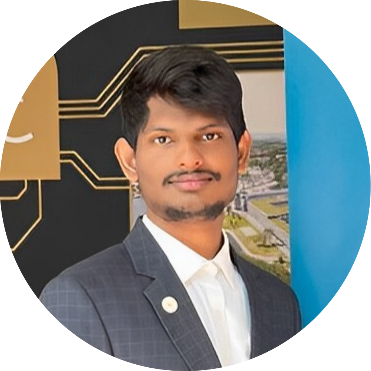
\includegraphics[width=2.7cm,clip]{images/resume_pic_m.png}}
}
\parbox{\dimexpr\linewidth-3.8cm\relax}{
\vspace{-20pt}
\begin{tabularx}{\linewidth}{L r} \\
    {\Huge \scshape  Venkata Sai Yakkshit Reddy Asodi}~
    \href{https://www.cedzlabs.com/yakkshit}{\vspace{1pt}}\\
      Berlin, Germany. \\ \vspace{1pt}
     \small \raisebox{-0.1\height}\faPhone\ +91 8179936156 ~ \href{mailto:saiyakkshit2001@gmail.com}{\raisebox{-0.2\height}\faEnvelope\  {saiyakkshit2001@gmail.com}} ~ 
    \href{https://linkedin.com/in/yakkshit/}{\raisebox{-0.2\height}\faLinkedin\ {yakkshit}}  ~
    \href{https://yakkshit.com/}{\raisebox{-0.2\height}\faGlobe\ {yakkshit.com}}  ~
    \href{https://github.com/yakkshit}{\raisebox{-0.2\height}\faGithub{ yakkshit}}
    \vspace{-8pt}
\end{tabularx}
}
\end{center}

\vspace{-23pt}
%-----------SUMMARY-----------
\section{Summary \faLink}
Full Stack Developer with expertise in Python and modern web frameworks, specialized in developing user interfaces for complex technical applications. Strong background in creating intuitive platforms for AI and computer vision solutions. Passionate about robotics and automation, with experience in building scalable applications that bridge hardware and software components. Demonstrated ability to work in fast-paced startup environments and collaborate with cross-functional teams.
\vspace{-10pt}
%-----------TECHNICAL SKILLS-----------
\section{\href{https://www.linkedin.com/in/yakkshit/details/skills/}{Technical Skills} \faLink}
\begin{itemize}[leftmargin=0.15in, label={}]
\small{\item{
\textbf{Languages - }{Python, JavaScript (ES6+), HTML5, CSS3} \\
\textbf{Frameworks - }{Vue.js, React, Django, Flask} \\
\textbf{Tools - }{Git, RESTful APIs, Docker, Computer Vision Libraries} \\
\textbf{Cloud \& Deployment - }{AWS, Azure, CI/CD Pipelines}\\
}}
\end{itemize}
\vspace{-15pt}

%-----------EXPERIENCE-----------
\section{Experience \faLinkedin}
\resumeSubHeadingListStart

\resumeSubheading
{\large Circleup AG \faBuilding}{December 2023 -- July 2024}
{Full Stack Engineer}{\faMapMarker \hspace{0.1cm} Zurich, Switzerland}\\
\vspace{10pt}
\textbf{Responsibilities:}
\resumeItemListStart
\vspace{-10pt}
\resumeItem{Developed and maintained a Python-based backend service for processing and analyzing complex data streams, integrating with multiple AI models and vision systems. Implemented RESTful APIs for seamless communication between frontend and backend services.}
\resumeItem{Created an intuitive web interface using Vue.js for monitoring and controlling automated systems. Built reusable components and implemented real-time data visualization for system metrics and performance monitoring.}
\resumeItemListEnd
\vspace{-3pt}
\textbf{Environment:}\emph{Python, Vue.js, Django, RESTful APIs, Docker}

\resumeSubheading
{Cedzlabs \faBuilding}{March 2023 -- July 2024}
{Full Stack Developer}{\faMapMarker \hspace{0.1cm} India}\\
\vspace{10pt}
\textbf{Responsibilities:}
\resumeItemListStart
\resumeItem{Built and maintained a web-based platform for computer vision applications using Python and Vue.js. Implemented user interface components for parameter configuration and real-time system monitoring. Collaborated with hardware teams to optimize software performance.}
\resumeItemListEnd
\vspace{-3pt}
\textbf{Environment:}\emph{Python, Vue.js, Flask, Computer Vision Libraries}
\vspace{-5pt}
%-----------PROJECTS-----------
\section{Projects \faGithub}
\resumeSubHeadingListStart

\resumeProjectHeading
{\textbf{\href{https://github.com/yakkshit/vision-platform}{Computer Vision Platform}} $|$ \emph{Python, Vue.js, OpenCV}}{December 2023}\\
\vspace{6pt}
\textbf{Description:}
\resumeItemListStart
\resumeItem{Developed a web-based platform for configuring and monitoring computer vision systems. Implemented a Python backend for image processing and analysis, with a Vue.js frontend for real-time visualization and control. Integrated with various vision sensors and processing pipelines.}
\resumeItemListEnd
\vspace{4pt}
\textbf{Tools:}\emph{Python, Vue.js, OpenCV, WebSocket, Docker}
\vspace{-5pt}
\resumeProjectHeading
{\href{https://github.com/yakkshit/automation-dashboard}{\textbf{Automation Control Dashboard}} $|$ \emph{Django, Vue.js}}{October 2023}\\
\vspace{6pt}
\textbf{Description:}
\resumeItemListStart
\resumeItem{Built a comprehensive dashboard for monitoring and controlling automated systems. Features included real-time status monitoring, system configuration management, and performance analytics. Implemented using Django backend and Vue.js frontend with WebSocket integration.}
\resumeItemListEnd
\vspace{4pt}
\textbf{Tools:}\emph{Django, Vue.js, Python, WebSocket, Docker}

%-----------ACHIEVEMENTS---------------
\section{Achievements / Contributions}
\resumeSubHeadingListStart
\resumeItemListStart
\resumeItem{Developed an open-source library for computer vision parameter optimization, gaining 200+ GitHub stars.}
\resumeItem{Led the implementation of a new deployment pipeline that reduced system setup time by 40\%.}
\resumeItem{Active contributor to Python-based automation and computer vision communities.}
\resumeItemListEnd

\resumeSubHeadingListEnd
\textbf{Strengths: }\emph{Problem-solving, system architecture, cross-functional collaboration, automation enthusiasm} \\
\textbf{Languages: }\emph{Telugu - Native $|$ English - Fluent $|$ Hindi - Fluent $|$ German - Elementary $|$ Swedish - Elementary}

\vspace{10pt}
\end{document}